\slajdid{02-s008}
\begin{frame}[label=02-s008]{Integrisana kola, čip i DIP kućište}
% element: 02-s008:e01
Standardna logička kola dostupna su kao integrisane komponente.\par
\textbf{SSI} (\emph{Small Scale Integration}): do 100 komponenti, odnosno oko 10 gejtova u jednom čipu.\par
Gejt je standardno logičko kolo.
\par\vspace{3mm}
% element: 02-s008:e02
\begin{columns}[T,onlytextwidth]
\begin{column}{.24\textwidth}\centering
\Oznaka{Čip}\par\vspace{3mm}
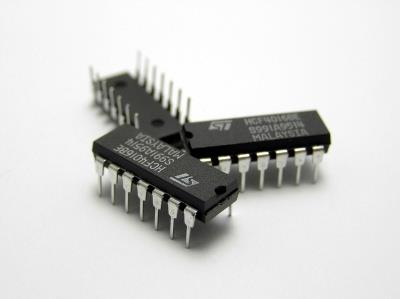
\includegraphics[width=.78\linewidth]{slike/izvorne/s008_integrisana_kola.jpg}
\par\vspace{1mm}
% element: 02-s008:e03
\Oznaka{\(1\,\mathrm{inch}=25{,}4\,\mathrm{mm}\)\\[1mm]
\(1\,\mathrm{mil}=10^{-3}\,\mathrm{inch}\)}
\end{column}
\begin{column}{.37\textwidth}\centering
\Oznaka{Raspored priključaka}\par\vspace{2mm}
\makebox[\linewidth][c]{% Pogled odozgo: četiri dvoulazna I kola u DIP-14 kućištu.
% Svaki vod se završava na odgovarajućem fizičkom pinu; napajanje i masa
% ostaju posebni priključci kućišta, bez prikaza unutrašnjih naponskih vodova.
\begin{tikzpicture}[font=\fontsize{9}{10.5}\selectfont,x=8mm,y=5.5mm,
  DEunutrasnje/.style={and gate US,draw,logic gate inputs=nn,
    minimum width=6mm,minimum height=5mm}]
% Zarez je deo spoljne konture, ne dodatna linija preko kućišta.
\draw[DEvod] (0,0)--(3.6,0)--(3.6,6)--(2.1,6)
 arc[start angle=0,end angle=-180,x radius=2.4mm,y radius=1.5mm]
 --(0,6)--cycle;
\foreach \pin/\oznaka [count=\k] in
 {1/A_0,2/B_0,3/O_0,4/A_1,5/B_1,6/O_1,7/\mathrm{GND}}{
  \pgfmathsetmacro{\visina}{5.55-.78*(\k-1)}
  \coordinate (p\pin) at (0,\visina);
  \draw[DEvod] (p\pin)--(-.3,\visina);
  \node[anchor=east,inner sep=1pt] at (-.38,\visina) {\(\pin\)};
  \node[anchor=east,inner sep=1pt] at (-.85,\visina) {\(\oznaka\)};
}
\foreach \pin/\oznaka [count=\k] in
 {14/V_{\mathrm{CC}},13/A_2,12/B_2,11/O_2,10/A_3,9/B_3,8/O_3}{
  \pgfmathsetmacro{\visina}{5.55-.78*(\k-1)}
  \coordinate (p\pin) at (3.6,\visina);
  \draw[DEvod] (p\pin)--(3.9,\visina);
  \node[anchor=west,inner sep=1pt] at (3.98,\visina) {\(\pin\)};
  \node[anchor=west,inner sep=1pt] at (4.5,\visina) {\(\oznaka\)};
}
\node[DEunutrasnje] (g0) at (1.05,5.13) {};
\node[DEunutrasnje] (g1) at (1.05,2.79) {};
\node[DEunutrasnje,rotate=180] (g2) at (2.55,4.35) {};
\node[DEunutrasnje,rotate=180] (g3) at (2.55,2.01) {};
% Leva dva kola: 1,2 -> 3 i 4,5 -> 6.
\draw[DEvod] (p1)--(.5,5.55)|-(g0.input 1);
\draw[DEvod] (p2)--(.5,4.77)|-(g0.input 2);
\draw[DEvod] (g0.output)--(1.7,5.13)|-(p3);
\draw[DEvod] (p4)--(.5,3.21)|-(g1.input 1);
\draw[DEvod] (p5)--(.5,2.43)|-(g1.input 2);
\draw[DEvod] (g1.output)--(1.7,2.79)|-(p6);
% Desna dva kola: 13,12 -> 11 i 10,9 -> 8.
% Redosled dva ulaza na istom I kolu je električno ravnopravan.
\draw[DEvod] (p13)--(3.24,4.77)|-(g2.input 2);
\draw[DEvod] (p12)--(3.24,3.99)|-(g2.input 1);
\draw[DEvod] (g2.output)--(1.9,4.35)|-(p11);
\draw[DEvod] (p10)--(3.24,2.43)|-(g3.input 2);
\draw[DEvod] (p9)--(3.24,1.65)|-(g3.input 1);
\draw[DEvod] (g3.output)--(1.9,2.01)|-(p8);
\end{tikzpicture}
}
\end{column}
\begin{column}{.04\textwidth}\end{column}
\begin{column}{.31\textwidth}\centering
\Oznaka{14-pinski DIP}\par
\makebox[\linewidth][c]{\begin{tikzpicture}[font=\fontsize{9}{10.5}\selectfont,x=1.7mm,y=1.04mm]
% Pogled odozgo, 14 izvoda.
\draw[DEvod] (0,15)--(0,18.1) arc[start angle=-90,end angle=90,radius=.45]--(0,22.11)--(19.94,22.11)--(19.94,15)--cycle;
\foreach \i in {0,...,6}{
 \pgfmathsetmacro{\x}{2.0+2.54*\i}
 \draw[DEvod] (\x,15)--++(0,-.5)--++(1.25,0)--++(0,.5);
 \draw[DEvod] (\x,22.11)--++(0,.5)--++(1.25,0)--++(0,-.5);
 \pgfmathtruncatemacro{\n}{\i+1}
 \node[DEcrvena,below,inner sep=1pt] at (\x+.625,14.5) {\n};
 \pgfmathtruncatemacro{\n}{14-\i}
 \node[DEcrvena,above,inner sep=1pt] at (\x+.625,22.61) {\n};
}
\draw[DEcrvena] (20.3,15)--(23.5,15) (20.3,22.11)--(23.5,22.11);
\draw[DEcrvena,<->] (22.7,15)--(22.7,22.11) node[midway,right,inner sep=1pt] {7.11};
% Bočni pogled i dimenzije iz originala.
\begin{scope}[yshift=-4mm]
\draw[DEvod] (0,4)--(0,8.5)--(19.94,8.5)--(19.94,4);
\draw[DEvod] (0,6.5)--(19.94,6.5);
\foreach \i in {0,...,6}{
 \pgfmathsetmacro{\x}{1.9+2.54*\i}
 \draw[DEvod,fill=white] (\x,4)--(\x,6.2)--++(.4,.3)--++(1.0,0)--++(.35,-.3)--++(0,-2.2)--++(-.4,-.5)--++(0,-2.6)--++(-.95,0)--++(0,2.6)--cycle;
}
\draw[DEcrvena] (0,8.8)--(0,11) (19.94,8.8)--(19.94,11);
\draw[DEcrvena,<->] (0,10.3)--(19.94,10.3) node[midway,above,inner sep=1pt] {19.94};
\draw[DEcrvena] (20.3,8.5)--(24,8.5) (20.3,3.42)--(24,3.42);
\draw[DEcrvena,<->] (23,3.42)--(23,8.5) node[midway,right,inner sep=1pt] {5.08};
\draw[DEcrvena] (20.3,.88)--(24,.88);
\draw[DEcrvena,<->] (21.5,.88)--(21.5,3.42) node[midway,right,xshift=1.5mm,inner sep=1pt] {2.54};
\draw[DEcrvena] (2.775,.5)--(2.775,-2) (5.315,.5)--(5.315,-2);
\draw[DEcrvena,<->] (2.775,-1.5)--(5.315,-1.5);
\node[DEcrvena,below,inner sep=1pt] at (4.045,-2.5) {2.54};

\end{scope}
\end{tikzpicture}
}
\end{column}
\end{columns}
\par\vspace{1mm}
% element: 02-s008:e04
\Oznaka{Ekonomski faktor: nabavka iste vrste čipa može biti isplativija.}
\end{frame}
